% Options for packages loaded elsewhere
\PassOptionsToPackage{unicode}{hyperref}
\PassOptionsToPackage{hyphens}{url}
%
\documentclass[
  a4paper,
]{article}
\usepackage{amsmath,amssymb}
\usepackage{setspace}
\usepackage{iftex}
\ifPDFTeX
  \usepackage[T1]{fontenc}
  \usepackage[utf8]{inputenc}
  \usepackage{textcomp} % provide euro and other symbols
\else % if luatex or xetex
  \usepackage{unicode-math} % this also loads fontspec
  \defaultfontfeatures{Scale=MatchLowercase}
  \defaultfontfeatures[\rmfamily]{Ligatures=TeX,Scale=1}
\fi
\usepackage{lmodern}
\ifPDFTeX\else
  % xetex/luatex font selection
\fi
% Use upquote if available, for straight quotes in verbatim environments
\IfFileExists{upquote.sty}{\usepackage{upquote}}{}
\IfFileExists{microtype.sty}{% use microtype if available
  \usepackage[]{microtype}
  \UseMicrotypeSet[protrusion]{basicmath} % disable protrusion for tt fonts
}{}
\makeatletter
\@ifundefined{KOMAClassName}{% if non-KOMA class
  \IfFileExists{parskip.sty}{%
    \usepackage{parskip}
  }{% else
    \setlength{\parindent}{0pt}
    \setlength{\parskip}{6pt plus 2pt minus 1pt}}
}{% if KOMA class
  \KOMAoptions{parskip=half}}
\makeatother
\usepackage{xcolor}
\usepackage[margin=1in]{geometry}
\usepackage{graphicx}
\makeatletter
\def\maxwidth{\ifdim\Gin@nat@width>\linewidth\linewidth\else\Gin@nat@width\fi}
\def\maxheight{\ifdim\Gin@nat@height>\textheight\textheight\else\Gin@nat@height\fi}
\makeatother
% Scale images if necessary, so that they will not overflow the page
% margins by default, and it is still possible to overwrite the defaults
% using explicit options in \includegraphics[width, height, ...]{}
\setkeys{Gin}{width=\maxwidth,height=\maxheight,keepaspectratio}
% Set default figure placement to htbp
\makeatletter
\def\fps@figure{htbp}
\makeatother
\setlength{\emergencystretch}{3em} % prevent overfull lines
\providecommand{\tightlist}{%
  \setlength{\itemsep}{0pt}\setlength{\parskip}{0pt}}
\setcounter{secnumdepth}{-\maxdimen} % remove section numbering
\ifLuaTeX
\usepackage[bidi=basic]{babel}
\else
\usepackage[bidi=default]{babel}
\fi
\babelprovide[main,import]{catalan}
% get rid of language-specific shorthands (see #6817):
\let\LanguageShortHands\languageshorthands
\def\languageshorthands#1{}
\ifLuaTeX
  \usepackage{selnolig}  % disable illegal ligatures
\fi
\usepackage{bookmark}
\IfFileExists{xurl.sty}{\usepackage{xurl}}{} % add URL line breaks if available
\urlstyle{same}
\hypersetup{
  pdfauthor={@tofermos 2024},
  pdflang={ca-ES},
  hidelinks,
  pdfcreator={LaTeX via pandoc}}

\title{Introducció a l'interface gràfic de Windows 11}
\author{@tofermos 2024}
\date{}

\begin{document}
\maketitle

{
\setcounter{tocdepth}{2}
\tableofcontents
}
\setstretch{1.5}
\newpage

\renewcommand\tablename{Tabla}

\section{1 UNITATS}\label{unitats}

Per accedir a qualsevol directori en Windows podem usar unes etiquetes
(lletres) que indiquen un inici de ruta. Esta lletra pot indicar.

\begin{enumerate}
\def\labelenumi{\arabic{enumi}.}
\tightlist
\item
  Una unitat física de memòria secundària: disc dur, pen-drive, tarja
  externa, DVD\ldots{}
\item
  Una partició d'una unitat fisica de memòria secundaria.
\item
  Una carpeta compartida en un xarxa.
\end{enumerate}

\subsection{1.1 Unitats físiques.}\label{unitats-fuxedsiques.}

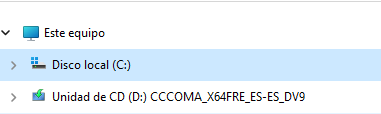
\includegraphics{png/unitatsDiscos.png}

\subsection{1.2 Particions}\label{particions}

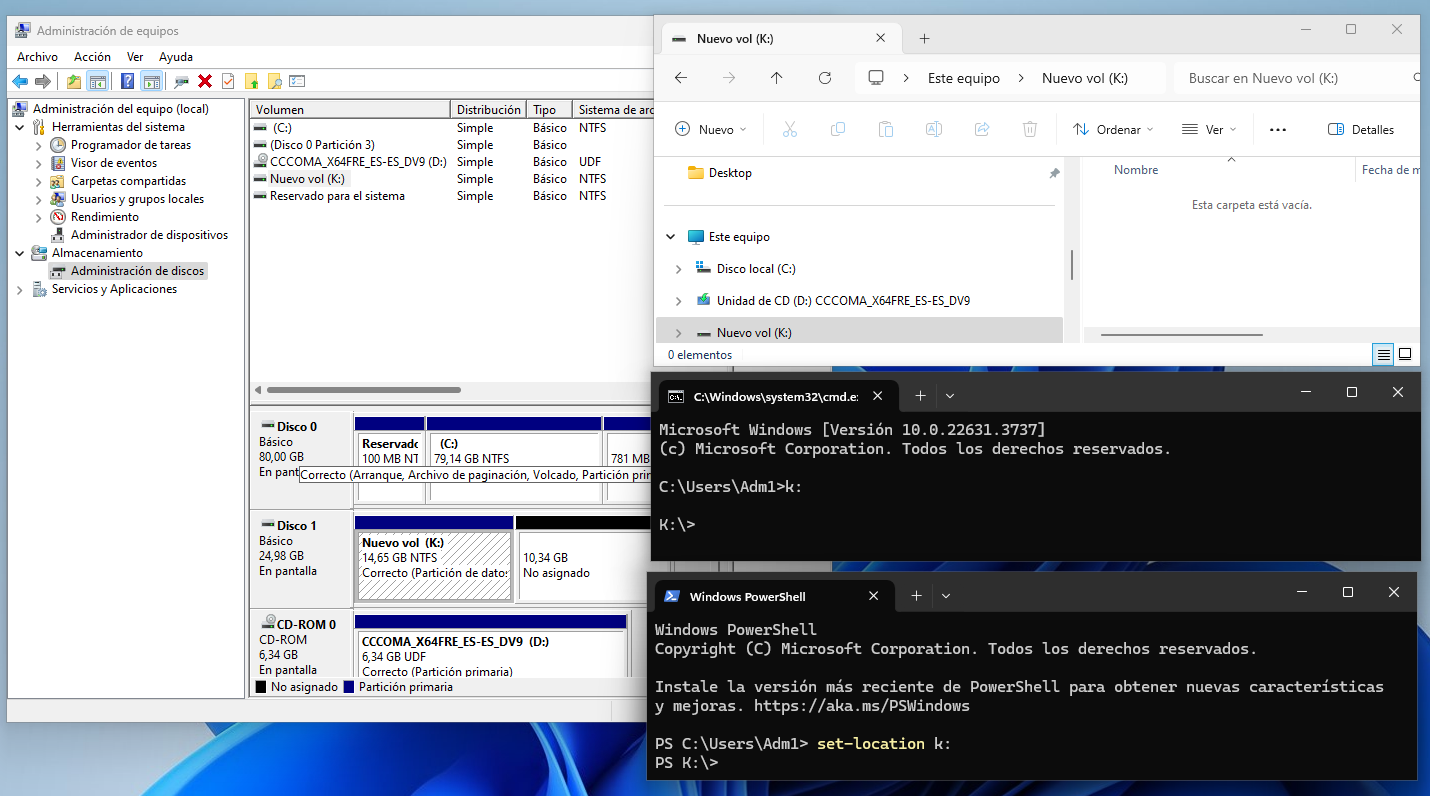
\includegraphics{png/unitatFormatejada.png}

\subsection{1.3 Carpetes compartides}\label{carpetes-compartides}

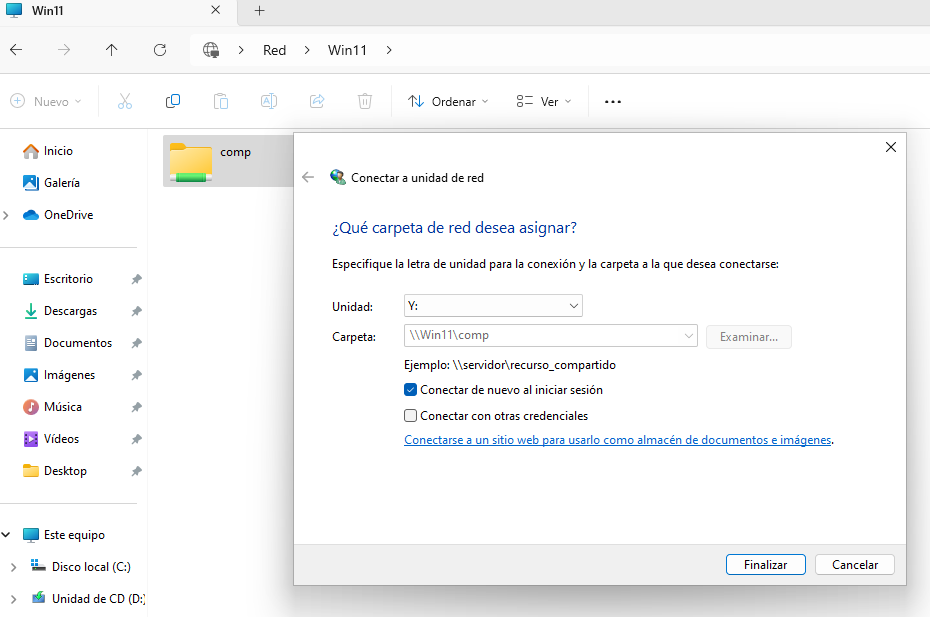
\includegraphics{png/conectarUnitat.png}

\textbf{Avanç}

\begin{quote}
En Windows quan per indicar la ubicació d'un fitxer o carpeta comencem
per una unitat, parlarem de \emph{rutes absolutes}. Alguns exemples
serien: \emph{C:\textbackslash Windows};
\emph{F:\textbackslash ParticioDades\textbackslash CopiaDeSeguretat};*
Z:\textbackslash UnitatDeXarxa\textbackslash FacturesAntigues*
\end{quote}

\section{2 OPCIONS DE L'EXPLORADOR}\label{opcions-de-lexplorador}

L'explorador de Windows és molt versàtil. Ens permet configurar la vista
per mostrar-nos i amagar-nos característiques del sistema de fitxers.
Abans de passar al següents punts necessitem canviar alguna configuració
de la vista que ens ve per defecte. Primer escollirem una vista que ens
mostre informació sobre els fitxers i carpetes (metadades).

\subsection{2.1 Vista de detalls o
metadades}\label{vista-de-detalls-o-metadades}

En l'opció VER triem Detalles

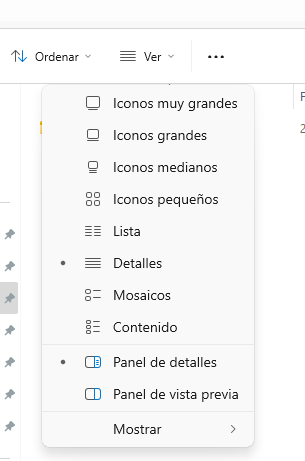
\includegraphics{png/verVistaDetalle0.png}

\subsection{2.2 Mostrar ocults i
extensions}\label{mostrar-ocults-i-extensions}

En l'opció ``Ver'' de cada carpeta, podem triar què volem que ens mostre
o oculte. Veiem dos canvis convenients per poder treballar com a
``Administradors''.

\begin{itemize}
\tightlist
\item
  Veure tots els fitxers i carpetes ocultes.
\item
  Veure totes les extensions dels fitxers.
\end{itemize}

En els \textbf{\ldots{}} desplegar i triar \emph{Opciones}

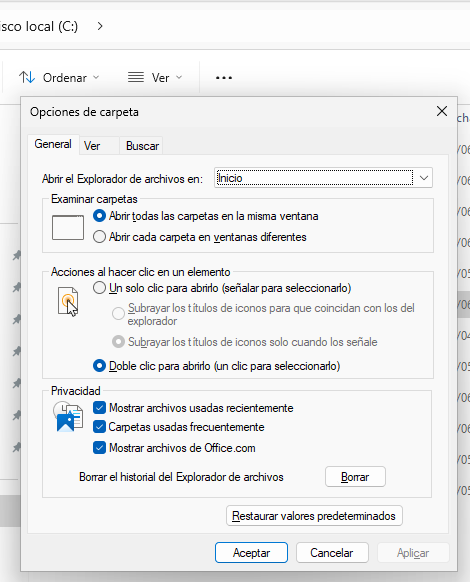
\includegraphics{png/verOpcionesdecarpeta1.png}

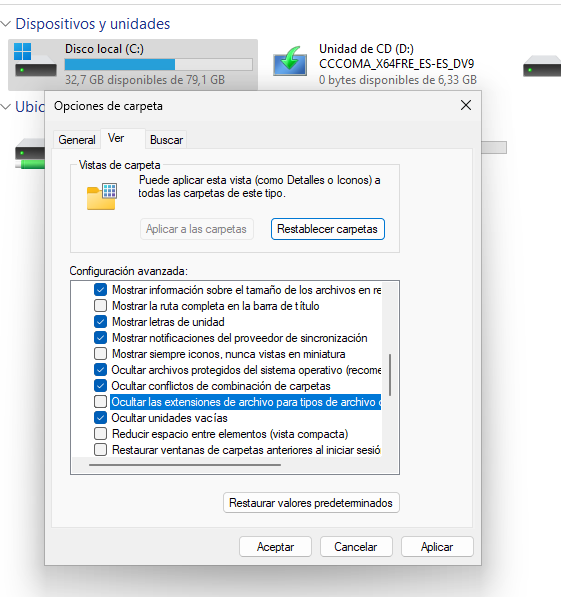
\includegraphics{png/verOpcionesdecarpeta2.png}

Podem fer el canvi sobre tota la Unitat o sobre una carpeta. Encara que
amb ``Aplicar a las carpetas'' també s'aplicaria a tota la unitat.

\subsection{2.3 Detalls o característiques a
mostrar}\label{detalls-o-caracteruxedstiques-a-mostrar}

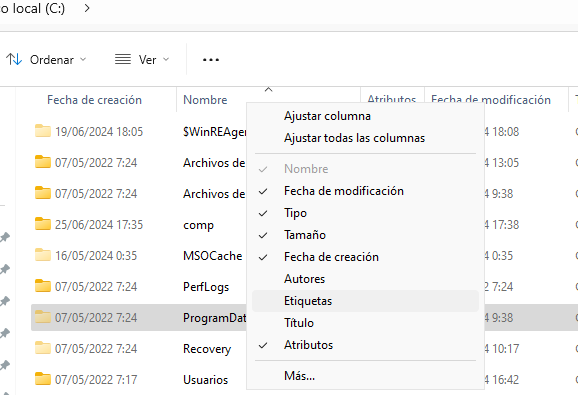
\includegraphics{png/verVistaDetalle.png}

\section{3. CARPETES PRINCIPALS de WINDOWS
11}\label{carpetes-principals-de-windows-11}

\subsection{3.1 PER DEFECTE}\label{per-defecte}

En la instal·lació de Windows 11 s'hi creen les carpetes principals
següents:

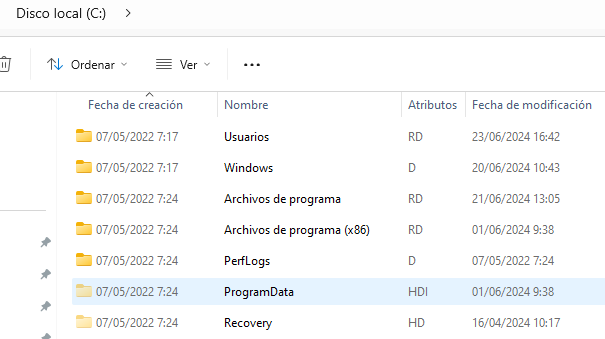
\includegraphics{png/carpetesPrincipals.png}

Les funcions són:

\begin{itemize}
\tightlist
\item
  \textbf{C:\textbackslash Windows} Conté els arxius del sistema
  operatiu Windows.
\item
  \textbf{C:\textbackslash Program Files} Conté els programes
  instal·lats (per a aplicacions de 64 bits).
\item
  \textbf{C:\textbackslash Program Files} (x86): Conté els programes
  instal·lats (per a aplicacions de 32 bits).
\item
  \textbf{C:\textbackslash Users} Conté les carpetes dels usuaris,
  incloent-hi documents, escriptori, descàrregues, etc.
\item
  \textbf{C:\textbackslash ProgramData} Emmagatzema les dades de les
  aplicacions compartides entre tots els usuaris del sistema.
\item
  \textbf{C:\textbackslash PerfLogs} Conté els registres de rendiment i
  diagnòstic del sistema.
\item
  \textbf{C:\textbackslash Recovery} Emmagatzema els arxius necessaris
  per a la recuperació del sistema.
\end{itemize}

\subsection{3.2 NOVES CARPETES}\label{noves-carpetes}

A la unitat C:\textbackslash{} poden crear-se'n més en funció de
posteriors configuracions i instal·lacions.

Per exemple:

\begin{itemize}
\tightlist
\item
  Si activem la recuperació del sistema es crea la carpeta
  \textbf{C:\textbackslash\$Recycle.bin}
\item
  Si instal·lem el MS Office s'hi crea
  \textbf{C:\textbackslash MSOCache}
\end{itemize}

\textbf{Notes}

\begin{quote}
\begin{itemize}
\tightlist
\item
  El ``\$'' com a inici de no de carpeta és una forma d'ocultar la
  carpeta.
\item
  Si no tenim habilitada l'opció de mostrar carpetes i arxius ocults
  (com hem vist adés) no veiem estes carpetes.
\item
  Hi ha altra forma d'ocultar amb atributs que estudiarem més avant.
\end{itemize}
\end{quote}

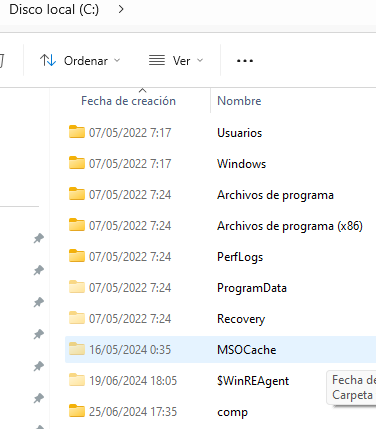
\includegraphics{png/carpetesPrincipalsCreadesDespres.png}

\section{4. PAPERERA DE RECICLATGE}\label{paperera-de-reciclatge}

Quan eliminem un fitxer o carpeta d'una unitat local, amb la
configuració per defecte, encara el podem recuperar perquè s'hi queda a
la \emph{Paperera de reciclatge}.

\subsection{4.1 Configuració}\label{configuraciuxf3}

Veiem què podem configurar a la paperera:

\begin{itemize}
\tightlist
\item
  Màxima quantitat d'informació o tamany.
\item
  Desactivar-la per que l'eliminació siga definitiva (equival a polsar
  SHIFT + Suprimir).
\item
  Mostrar un avís de confirmació abans de la supressió.
\end{itemize}

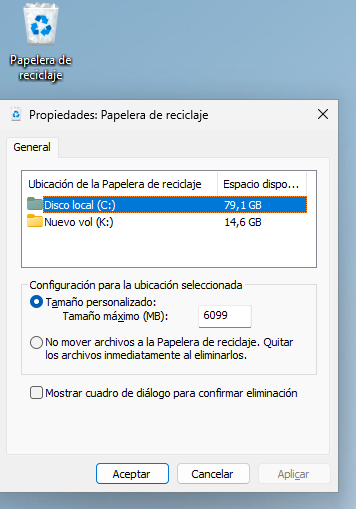
\includegraphics{png/paperera.png}

\subsection{4.2 Recuperació}\label{recuperaciuxf3}

Veiem dos vistes distintes del contingut.

Per recuperar un arxiu o carpeta eliminat, obrim la paperera dels del
GUI i amb botó contrari donem RESTAURAR

Des del CLI també es pot. Ho vorem més avant.

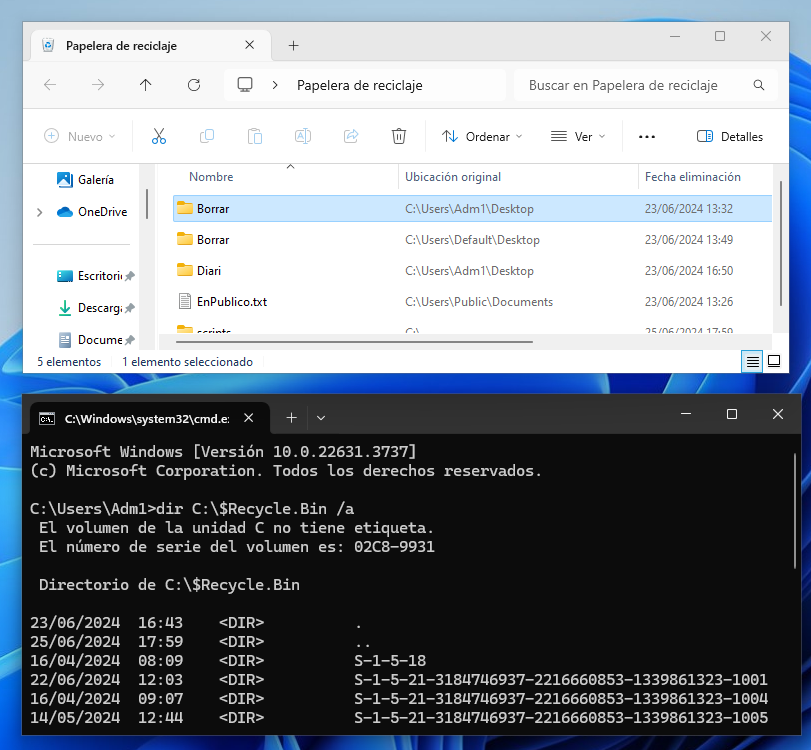
\includegraphics{png/paperera1.png}

\textbf{Advertència} \textgreater{} Encara que treballem en
instal·lacions locals i no ens afecta, convé recordar que si
l'eliminació de fitxer de la xarxa no van a la paperera. S'eliminen
directament.

\textbf{Avanç} \textgreater Una tasca interessant quan s'estudies la
programació de tasques seria la de programar un buidat periòdic de la
paperera.

\section{5 DRECERES}\label{dreceres}

Existeixen algunes combinacions de tecles ( Dreceres ) que ens permeten
realitzar accions de manera ràpida i eficient, sense necessitat d'usar
el ratolí.

\subsection{5.1 Drecres comunes}\label{drecres-comunes}

\begin{itemize}
\tightlist
\item
  \textbf{Ctrl + C}: Copiar.
\item
  \textbf{Ctrl + X}: Tallar.
\item
  \textbf{Ctrl + V}: Enganxar.
\item
  \textbf{Ctrl + Z}: Desfer.
\item
  \textbf{Ctrl + Y}: Repetir.
\item
  \textbf{Ctrl + A}: Seleccionar tot.
\item
  \textbf{Ctrl + S}: Desar.
\item
  \textbf{Ctrl + P}: Imprimir.
\item
  \textbf{Ctrl + N}: Nou (crea un nou document o finestra, depenent de
  l'aplicació).
\item
  \textbf{Ctrl + F}: Buscar.
\item
  \textbf{Alt + Tab}: Canviar entre les aplicacions obertes.
\item
  \textbf{Alt + F4}: Tancar la finestra activa.
\item
  \textbf{F2}: Canviar el nom de l'element seleccionat.
\item
  \textbf{F5}: Actualitzar la finestra activa.
\item
  \textbf{Esc}: Cancel·lar l'acció actual.
\end{itemize}

\subsection{5.2 Dreceres específiques de
Windows}\label{dreceres-especuxedfiques-de-windows}

\begin{itemize}
\tightlist
\item
  \textbf{Windows + D}: Mostra o amaga l'escriptori.
\item
  \textbf{Windows + E}: Obre l'Explorador de Fitxers.
\item
  \textbf{Windows + L}: Bloqueja el PC.
\item
  \textbf{Windows + R}: Obre el quadre de diàleg Executar.
\item
  \textbf{Windows + I}: Obre la configuració de Windows.
\item
  \textbf{Windows + Tab}: Obre la Vista de Tasques.
\item
  \textbf{Windows + A}: Obre el Centre d'Acció.
\item
  \textbf{Windows + S} o \textbf{Windows + Q}: Obre la cerca.
\item
  \textbf{Windows + X}: Obre el menú d'accés ràpid (menú d'inici ràpid).
\item
  \textbf{Windows + V}: Obre l'historial del porta-retalls.
\item
  \textbf{Windows + P}: Projectar la pantalla (canviar mode de
  visualització).
\end{itemize}

\subsection{5.3 Drecreres per a la gestió de
finestres}\label{drecreres-per-a-la-gestiuxf3-de-finestres}

\begin{itemize}
\tightlist
\item
  \textbf{Windows + Fletxa esquerra/dreta}: Anclar la finestra activa a
  la meitat esquerra o dreta de la pantalla.
\item
  \textbf{Windows + Fletxa amunt/avall}: Maximitzar o minimitzar la
  finestra activa.
\item
  \textbf{Windows + Maj + Fletxa esquerra/dreta}: Moure la finestra
  activa al monitor esquerre o dret en una configuració de monitors
  múltiples.
\end{itemize}

\subsection{5.4 Dreceres de la terminal de
Windows}\label{dreceres-de-la-terminal-de-windows}

\begin{itemize}
\tightlist
\item
  \textbf{Ctrl + Maj + N}: Obre una nova finestra de la Terminal amb
  privilegis d'administrador.
\item
  \textbf{Ctrl + Maiúscules + T}: Obre una nova pestanya a la Terminal.
\end{itemize}

\subsection{5.5 Dreceres
personalitzades}\label{dreceres-personalitzades}

Pots crear les teues dreceres per a aplicacions específiques:

\begin{enumerate}
\def\labelenumi{\arabic{enumi}.}
\tightlist
\item
  Fes clic amb el botó dret sobre la icona de l'aplicació i selecciona
  ``Propietats''.
\item
  A la pestanya ``Accés directe'', trobaràs el camp ``Tecla de
  drecera''.
\item
  Fes clic al camp i pressiona la combinació de tecles que vols assignar
  com a drecera.
\end{enumerate}

L'ús de la drecera \textbf{Windows + R} ens servirà per introduir el
concepte de Variables del Sistema i concretament la variable
\textbf{PATH}.

\end{document}
